\chapter[Implementación]{Implementación}
\label{Chap5}

\section{Entorno de ejecución}
El proyecto se dividirá en dos ordenadores (maquinas virtuales). Uno de ellos será el responsable de la base de datos en PostGreSQL, mientras que, el otro, se encargara de la ejecución del código de obtención de datos, tratarlos y enviarlos a la base de datos.

\subsection{Preparación de entorno virtual}
Primero instalaremos las dependencias para crear y activar un entorno virtual sobre el que trabajar, para ello se deben ejecutar los comandos mostrados en código \ref{cod:88}.

\begin{lstlisting}[caption={Instrucciones por consola para la creacion de un entrono virtual}, label=cod:88]
	#Instalamos las dependencias
	user@host:~$ sudo apt install python3-venv python3-dev
	
	#Creamos un nuevo directorio sobre el que trabajar
	user@host:~$ mkdir ~/dirdemiproyecto
	user@host:~$ cd ~/dirdemiproyecto
	
	#Creamos el entorno virtual
	user@host:~/dirdemiproyecto$ python3 -m venv envdemiproyecto
	
	#Activamos el entorno virtual
	user@host:~/dirdemiproyecto$ source envdemiproyecto/bin/activate
	
	#Una vez seguidos los pasos nuestra terminal debe mostrarse asi
	(envdemiproyecto) user@host:~/dirdemiproyecto$
\end{lstlisting}

Cada Spider dispondrá de su propio entorno virtual, nombrado tras la pagina web a la que representa, de esta forma, por ejemplo, el entorno virtual para la web de CHcantábrico se llamará chcantabrico. Otro entorno virtual es usado para el servidor Django y los scripts encargados del envío de datos.

\subsection{Instalación y configuración de PostGreSQL}
Los comandos necesarios para la instalación inicial de PostGreSQL, la creación de un usuario y una base de datos están presentes en código \ref{cod:89}.

\begin{lstlisting}[caption={Instrucciones por consola para iniciar una base de datos en PostGreSQL}, label=cod:89]
	#Instalamos PostGreSQL y las dependencias
	user@host:~$ sudo apt install libpq-dev postgresql postgresql-contrib
	
	#Iniciamos sesion usando el role postgres y accedemos a PostGreSQL
	user@host:~$ sudo -u postgres psql
	
	#Si todo esta bien la terminal deberia mostrarse asi
	postgres=# 
	
	#Creamos un nuevo usuario
	postgres=# CREATE USER miusuario WITH PASSWORD 'micontrasena';
	
	#Configuramos varios parametros del usuario para una mejor integracion con Django
	postgres=# ALTER ROLE miusuario SET client_encoding TO 'utf8';
	postgres=# ALTER ROLE miusuario SET default_transaction_isolation TO 'read committed';
	postgres=# ALTER ROLE miusuario SET timezone TO 'Europe/Madrid';
	
	#Creamos la Base de Datos
	postgres=# CREATE DATABASE bbddmiproyecto;
	
	#Otorgamos permisos de administrador a nuestro usuario en la base de datos
	postgres=# GRANT ALL PRIVILEGES ON DATABASE bbddmiproyecto TO miusuario;
	
	#Una vez finalizado
	postqres=# \q
\end{lstlisting}

En este punto ya se dispondría de una base de datos (aun sin tablas en ella) y de un usuario con el que conectarse a esta desde Django. Ahora quedaría configurar el permiso de comunicación entre dispositivos, más concretamente la conexión remota de Django con PostGreSQL. Los pasos a seguir se muestra en código \ref{cod:90}.

\begin{lstlisting}[caption={Instrucciones por consola y editor de texto para permitir la conexión remota en PostGreSQL}, label=cod:90]
	#Abrimos el archivo postgresql.conf con un editor
	user@host:~$ sudo nano /etc/postgresql/11/main/postgresql.conf
	
	#Buscamos la linea "#listen_addresses = 'localhost'", borramos la almohadilla y
	sustituimos localhost por *, permitiendo la escucha de cualquier direccion IP
	listen_addresses = '*'
	
	#Guardamos y cerramos el fichero
	
	#Abrimos el archivo pg_hba.conf con un editor
	user@host:~$ sudo nano /etc/postgresql/11/main/pg_hba.conf
	
	#Por defecto solo permite conexiones desde localhost
	# IPv4 local connections: 
	host    all             all             127.0.0.1/32            md5 
	
	#Configuararemos el permiso de conexion remota desde cualquier IP anyadiendo
	la siguiente linea debajo de la anterior
	host    all             all             0.0.0.0/0            md5 
	
	#O podemos configurar el permiso unicamente para la IP de la otra maquina virtual
	host    all             all             127.18.83.198/19            md5 
	
	#Guardamos y cerramos el fichero
	
	#Finalmete permitimos el trafico mediante el puerto 5432 (puesto por defecto)
	user@host:~$ sudo ufw allow 5432/tcp
\end{lstlisting}

\subsection{Instalación y configuración de Django}
Antes de instalar y crear un proyecto en Django con los comandos en código \ref{cod:91}, es necesario generar un entorno virtual sobre el que trabajar como se muestra en código \ref{cod:88}.

\begin{lstlisting}[caption={Instrucciones por consola de instalación y creación de un proyecto en Django}, label=cod:91]
	#Instalamos Django y las dependencias
	(envdemiproyecto) user@host:~/dirdemiproyecto$ pip install django psycopg2
	
	#Creamos un nuevo proyecto de Django
	(envdemiproyecto) user@host:~/dirdemiproyecto$ django-admin startproject djangoAPI
	(envdemiproyecto) user@host:~/dirdemiproyecto$ cd djangoAPI
	
	#Creamos una nueva app Django
	(envdemiproyecto) user@host:~/dirdemiproyecto/djangoAPI$ python manage.py startapp appAPI
\end{lstlisting}

Una vez se dispone del proyecto y la app de Django, quedaría configurar la API, indicando la base de datos a usar y configurando la conexión remota en Django. Configuración presente en código \ref{cod:92}.

\begin{lstlisting}[caption={Instrucciones por consola y editor de texto para la configuración de la API Django}, label=cod:92]
	#Abrimos el archivo settings.py con un editor
	(envdemiproyecto) user@host:~/dirdemiproyecto/djangoAPI$ nano djangoAPI/settings.py
	
	#Anyadimos nuestra app en la lista de INSTALLED_APPS
	INSTALLED_APPS = [
		'django.contrib.admin',
		'django.contrib.auth',
		'django.contrib.contenttypes',
		'django.contrib.sessions',
		'django.contrib.messages',
		'django.contrib.staticfiles',
		'appAPI.apps.AppapiConfig',
	]
	
	#Configuramos la base de datos sutituyendo
	DATABASES = {
		'default': {
			'ENGINE': 'django.db.backends.sqlite3',
			'NAME': os.path.join(BASE_DIR, 'db.sqlite3'),
		}
	}
	
	por
	
	DATABASES = {
		'default': {
			'ENGINE': 'django.db.backends.postgresql_psycopg2',
			'NAME': 'bbddmiproyecto',
			'USER': 'miusuario',
			'PASSWORD': 'micontrasena',
			'HOST': '172.18.83.197',
			'PORT': '5432',
		}
	}
	
	#Configuramos las IP admitidas
	ALLOWED_HOSTS = ['172.18.83.197', 'localhost']
	
	#Configuramos la zona horaria
	TIME_ZONE = 'Europe/Madrid'
	
	#Configuramos el tamanyo maximo de datos a None, con el fin de poder
	enviar cualquier cantidad de datos
	DATA_UPLOAD_MAX_MEMORY_SIZE = None
	
	#Guardamos y cerramos el fichero
	
	#Finalmete permitimos el trafico mediante el puerto 8000 (puesto por defecto)
	user@host:~$ sudo ufw allow 8000
\end{lstlisting}

Tras configurar la API, toca crear los modelos de la base de datos. Primero se accede al archivo models.py con el comando indicado en código \ref{cod:93}. Inicialmente se encontrara vacio, por lo que  se incluye el código en \ref{cod:94}, definiendo los modelos Data y Code.

\begin{lstlisting}[caption={Instrucción por consola para abrir models.py en un editor de texto}, label=cod:93]
	#Abrimos el archivo models.py dentro de la carpeta appAPI con un editor
	(envdemiproyecto) user@host:~/dirdemiproyecto/djangoAPI$ nano appAPI/models.py
\end{lstlisting}

\begin{lstlisting}[language=Python, caption={Modelos API Django}, label=cod:94]
	from django.db import models
	
	class Data(models.Model):
		temperatura = models.FloatField(null=True)
		humedad = models.FloatField(null=True)
		precipitacion = models.FloatField(null=True)
		nivel = models.FloatField(null=True)
		caudal = models.FloatField(null=True)
		radiacion = models.FloatField(null=True)
		fecha = models.DateTimeField()
		estacion = models.ForeignKey("Code", on_delete=models.CASCADE)
	
	class Code(models.Model):
		estacion = models.CharField(max_length=50)
		codigo = models.CharField(max_length=20, primary_key=True)
		coodenadas = models.CharField(max_length=50)
		seguimiento = models.FloatField(null=True)
		prealerta = models.FloatField(null=True)
		alerta = models.FloatField(null=True)
\end{lstlisting}

Para importar los modelos a la base de datos, con el fin de crear las respectivas tablas, se requieren de los comandos en código \ref{cod:95}.

\begin{lstlisting}[caption={Instrucción por consola para abrir models.py en un editor de texto}, label=cod:95]
	#Actualizamos los datos realizados en models.py
	(envdemiproyecto) user@host:~/dirdemiproyecto$ python3 manage.py makemigrations
	
	#Migramos los datos
	envdemiproyecto) user@host:~/dirdemiproyecto$ python3 manage.py migrate
\end{lstlisting}

Si se quiere confirmar la correcta creación de las tablas, desde la terminal de PostGreSQL, se ejecutaran los comando de código \ref{cod:96}. Si todo a ido bien, se deberían mostrar como en la figura \ref{fig:ej34}.

\begin{lstlisting}[caption={Instrucción por consola para abrir models.py en un editor de texto}, label=cod:96]
	#Nos conectamos a la base de datos
	postgres=# \c bbddmiproyecto
	
	#Mostramos las tablas
	postgres=# \d
\end{lstlisting}

\begin{figure} [H]
	\centering
	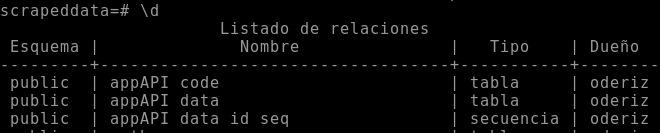
\includegraphics[width=0.6\textwidth]{fig/comprobacionTablasBBDD.png}
	\caption[Lista de tablas en PostGreSQL]{Lista de tablas en PostGreSQL}
	\label{fig:ej34}
\end{figure}

Tras configurar la API y crear las tablas de la base de datos, se creará la API como tal. Para ello se creara el archivo urls.py mediante el comando en código \ref{cod:97}. Dentro se incluye el código en \ref{cod:98}, que define las rutas para realizar una llamada a la API, en este caso storeData y storeCode.

\begin{lstlisting}[caption={Instrucción por consola para crear y abrir el fichero urls.py dentro de la carpeta de la app en un editor de texto}, label=cod:97]
	#Creamos el archivo urls.py con un editor dentro de la carpeta appAPI
	(envdemiproyecto) user@host:~/dirdemiproyecto/djangoAPI$ nano appAPI/urls.py
\end{lstlisting}

\begin{lstlisting}[language=Python, caption={Definición URLs API}, label=cod:98]
	from django.urls import path
	from django.views.decorators.csrf import csrf_exempt
	
	from . import views
	
	urlpatterns = [
	path("storeData", csrf_exempt(views.storeData), name="storeData"),
	path("storeCode", csrf_exempt(views.storeCode), name="storeCode"),
	]
\end{lstlisting}

Si se quiere que el proyecto tenga constancia de ellas. Se debe modificar el fichero urls.py incluido dentro de la carpeta del proyecto, por lo que se abre con el comando del código \ref{cod:99}. y se escribe el contenido de código \ref{cod:100}.

\begin{lstlisting}[caption={Instrucción por consola para abrir el fichero urls.py dentro de la carpeta del proyecto en un editor de texto}, label=cod:99]
	#Abrimos el archivo urls.py dentro de la carpeta djangoAPI con un editor
	(envdemiproyecto) user@host:~/dirdemiproyecto/djangoAPI$ nano djangoAPI/urls.py
\end{lstlisting}

\begin{lstlisting}[language=Python, caption={Configuración URLs API}, label=cod:100]
	from django.contrib import admin
	from django.urls import path, include
	
	urlpatterns = [
		path('admin/', admin.site.urls),
		path('appapi/', include('appapi.urls'))
	]
\end{lstlisting}

Para finalizar, se crean las vistas a las que dirigen las rutas dentro del archivo views.py, abriéndolo con el comando en código \ref{cod:101}. El archivo se encontrara vacio y, ce incluye el codigo en \ref{cod:102}. Estas funciones se encargan de recibir los datos enviados, iterar por ellos y subirlos a la base de datos con el método \textit{save()}. Concluyendo la creación y configuración de la API.

\begin{lstlisting}[caption={Instrucción por consola para abrir el fichero views.py dentro de la carpeta de la app en un editor de texto}, label=cod:101]
	#Abrimos el archivo views.py dentro de la carpeta appAPI con un editor
	(envdemiproyecto) user@host:~/dirdemiproyecto/djangoAPI$ nano appAPI/views.py
\end{lstlisting}

\begin{lstlisting}[language=Python, caption={Definición funciones de recepción y almacenamiento de datos API}, label=cod:102]
	import json
	
	from django.http import JsonResponse
	from .models import Data, Code
	
	# Create your views here.
	def storeData(request):
		data = json.loads(request.body.decode("utf-8"))
		for estacion in data:
			for datos in estacion['datos']:
				dato = Data(
					temperatura=datos['temperatura (C)'],
					humedad=datos['humedad (%)'],
					precipitacion=datos['precipitacion (mm)'],
					nivel=datos['nivel (m)'],
					caudal=datos['caudal (m^3/s)'],
					radiacion=datos['radiacion (W/m^2)'],
					fecha=datos['fecha y hora'],
					estacion=estacion['estacion']
				)
				dato.save()
		return JsonResponse(data, safe=False)
	
	def storeCode(request):
		data = json.loads(request.body.decode("utf-8"))
		for estacion in data:
			dato = Code(
				estacion=estacion['estacion'],
				codigo=estacion['codigo'],
				coodenadas=estacion['coodenadas'],
				seguimiento=estacion['seguimiento'],
				prealerta=estacion['prealerta'],
				alerta=estacion['alerta'],
			)
			dato.save()
	return JsonResponse(data, safe=False)
\end{lstlisting}

\section{Creación de Spiders}
Una vez instalado Scrapy, en el directorio escogido, se usa el comando \ref{cod:1} para generar un nuevo proyecto de Scrapy.

\begin{lstlisting}[caption={Instrucciones de consola en Linux para la creación de un proyecto scrapy}, label=cod:1]
	scrapy startproject miproyecto
\end{lstlisting}

El cual crea un nuevo directorio con el mostrado en la figura \ref{fig:ej11}.

\begin{figure} [h!]
	\centering
	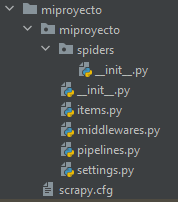
\includegraphics[width=0.3\textwidth]{fig/estructura_proyecto_scrapy.png}
	\caption[Pantalla del IDE donde se ve la estructura del proyecto]{Pantalla del IDE donde se ve la estructura del proyecto}
	\label{fig:ej11}
\end{figure}

En el directorio recientemente creado, se ejecuta el comando \ref{cod:2} encargado de crear la Spider.

\begin{lstlisting}[caption={Instrucciones de consola en Linux para la creación de una Spider scrapy}, label=cod:2]
	cd miproyecto
	scrapy genspider mispider webausar.com
\end{lstlisting}

En caso de no especificar el protocolo usado por la web, Scrapy asumirá que usa HTTPS. Tras ejecutar el comando la Spider habrá sido generada dentro de la carpeta spiders. Visto en la figura \ref{fig:ej12}.

\begin{figure} [h!]
	\centering
	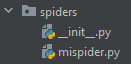
\includegraphics[width=0.2\textwidth]{fig/primera_spider.png}
	\caption[Directorio de almacenamiento de las Spider]{Directorio de almacenamiento de las Spider}
	\label{fig:ej12}
\end{figure}

Una vez abierto el archivo dispone del código \ref{cod:3}.

\begin{lstlisting}[language=Python, caption={Spider recién generada}, label=cod:3]
	import scrapy
	
	class MispiderSpider(scrapy.Spider):
		name = "mispider"
		allowed_domains = ["webausar.com"]
		start_urls = ["https://webausar.com"]
	
		def parse(self, response):
			pass
\end{lstlisting}

Scrapy usa una programación orientada a objetos, siendo cada Spider una clase representada dentro del proyecto.\newline
\newline
Analizando las variables definidas en el código \ref{cod:3} vemos las siguientes, \textit{name}, nombre por el que referenciar la Spider a la hora de ejecutarla; \textit{allowed\_domains}, indica que dominios están permitidos, es importante no especificar protocolo, de esta manera funcionara para cualquier web ya sea HTTP como HTTPS que pertenezca a ese dominio, de lo contrario se limitara al protocolo indicado; \textit{start\_urls}, URL inicial sobre la que se hará la request de petición de datos.\newline
\newline
El método \textit{parse()} es aquel al que se envía la respuesta obtenida de la web, para realizar el filtrado de la información deseada. Este método es invocado automáticamente por la Spider, sin necesidad real de hacerlo manualmente. Puede ser un método recursivo en caso de así quererlo o incluso se pueden definir nuevas funciones \textit{parse()} en caso de necesitarlas.

\subsection{Proceso de obtención de datos}
La extracción de los datos, requiere ir a la web deseada e inspeccionar su estructuración HTML. Para ello, como ejemplo, se va a usar la web de Aemet. Como muestra la figura \ref{fig:ej13}.

\begin{figure} [H]
	\centering
	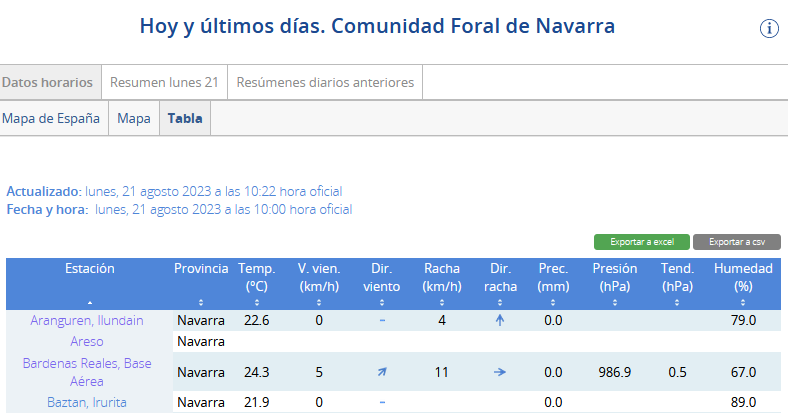
\includegraphics[width=0.8\textwidth]{fig/AemetCode.png}
	\caption[URL de inicio para obtener los códigos de las estaciones de Aemet]{Web de Aemet para obtención de datos}
	\label{fig:ej13}
\end{figure}

Accedes a la información en formato texto sin renderizar, se busca el elemento representativo de los datos deseados. En este caso, el nombre y código de la estación. Ambos se encuentran en el mismo elemento que forma la primera columna de la tabla. Como se ve en el código \ref{cod:4}

\begin{lstlisting}[caption={Estructura HTML de los datos deseados Aemet. Los puntos suspensivos de las líneas 10 y 12 representan código omitido.}, label=cod:4]
	<table id="table">
		<thead></thead>
		<tbody>
			<tr class="fila_par">
				<td>
					<a href="/es/eltiempo/observacion/ultimosdatos?k=nav&"
					"amp;l=9263X&amp;w=0&amp;datos=det&"
					"amp;f=precipitacion">Aranguren, Ilundain</a>
				</td>
				...
			</tr>
			...
		</tbody>
	</table>
\end{lstlisting}

En este caso es posible filtrar fácilmente los datos, obteniendo todos directamente, aunque lo más común sería obtener las filas primero para luego iterar por cada una de ellas. Para obtenerlos se puede hacer mediante el selector de XPath como con el de CSS.\newline
\newline
Ambos se pueden obtener fácilmente en la herramienta de inspección, una vez seleccionado el elemento deseado, click derecho sobre el y, en el apartado copiar se mostrará la posibilidad de copiar ambos selectores. Es probable que el selector proporcionado no sea del todo lo que se busque o se pueda simplificar, por lo que es recomendable comprobarlo manualmente. Visto en el código \ref{cod:5}.

\begin{lstlisting}[language=Python, caption={Selectores posibles para la obtención de los datos de código y nombre de estación en Aemet}, label=cod:5]
	rows = response.xpath('//div[@id="contenedor_tabla"]/table/tbody/tr/td/a')
	
	rows = response.css("div#contenedor_tabla tbody tr a")
\end{lstlisting}

Esto devuelve una lista de objetos tipo Selector, cosa que permite conforme se itera por cada elemento, volver a usar un selector para filtrar unicamente los datos deseados. En este caso, código \ref{cod:6} muestra esto.

\begin{lstlisting}[language=Python, caption={Selectores posibles para el filtrado de los datos de código y nombre de estación en Aemet}, label=cod:6]
	path = rows[i].xpath("@href").get()
	name = rows[i].xpath("./text()").get()
	
	path = rows[i].css("*::attr(href)").get()
	name = rows[i].css("*::text").get()
\end{lstlisting}

De esta forma, mediante el uso de la función \textit{get()}, se pasa de tener un objeto Selector a un String. El uso de \textit{get()} sobre una lista devuelve el primer elemento, en caso de querer transformar toda la lista el método a usar es \textit{getall()}.\newline
\newline
Finalmente, como de la URL obtenida,
\begin{verbatim}
	('/es/eltiempo/observacion/ultimosdatos?k=nav&l=9263X&w=0&datos=det&f=precipitacion')
\end{verbatim}
solo es de interés el código de la estación (parámetro l de la query empezando por 0), se filtra mediante \textit{split()}. Como se ve en el código \ref{cod:7}

\begin{lstlisting}[language=Python, caption={Filtrado del código de estación de la URL en Aemet}, label=cod:7]
	code = path.split('&')[1].split('=')[1]
\end{lstlisting}

\subsection{Guardado de datos}
Scrapy almacena los datos en forma de múltiples diccionarios, tantos como webs usadas. Para acceder a esta información Scrapy proporciona dos alternativas, el uso de \textit{Items} junto a \textit{ItemLoaders}, siendo clases especificas de Scrapy o, mediante la palabra reservada \textit{yield} de Python, que tiene una funcionalidad parecida a \textit{return}, siendo esta la opción elegida debido a su fácil implementación. Esto se muestra en el código \ref{cod:8}.

\begin{lstlisting}[language=Python, caption={Guardar datos mediante el uso de \textit{yield}}, label=cod:8]
	yield {
		'estacion': name,
		'codigo': path.split('&')[1].split('=')[1],
	}
\end{lstlisting}

Actualmente, si se ejecuta la Spider imprimirá los datos obtenidos por pantalla, aunque pueden ser almacenados en un fichero tanto CSV como JSON, a la hora de ejecutar la Spider añadiendo en el comando \textit{-o nombre.csv} ó \textit{-o nombre.json}.\newline
\newline
Para un uso ligero de forma manual, esa alternativa es más que suficiente, pero en este proyecto, como se quieren ejecutar de forma automática mediante el uso de Runners, se debe se implementar una variable llamada \textit{custom\_settings} para cada una de las Spider. Esta permite, sin la necesidad de modificar el archivo settings.py, añadir configuraciones o dependencias independientes en las Spiders. Se puede ver en el Código \ref{cod:9}.

\begin{lstlisting}[language=Python, caption={Confugurar guardado en JSON mediante \textit{custom\_settings}}, label=cod:9]
	custom_settings = {
		'FEEDS': {
			'JSONs/RawCode/codigos_aemet.json': {
				'format': 'json',
				'encoding': 'utf-8',
				'overwrite': True,
			}
		}
	}
\end{lstlisting}

Indicando que, en la ruta que se especifica, almacene un fichero JSON utf-8 y, que cada vez que se llame a esta Spider sobre-escriba el fichero anterior.

\subsection{Spider básica}
Tras realizar los pasos, esta es la Spider básica terminada.

\begin{lstlisting}[language=Python, caption={Spider de ejemplo (Aemet Code Spider)}]
	import scrapy
	
	
	class AemetCodeSpider(scrapy.Spider):
		name = "aemet_code"
		allowed_domains = ["www.aemet.es"]
		start_urls = ["https://www.aemet.es/es/eltiempo/observacion/"
		"ultimosdatos?k=nav&w=0&datos=det&x=h24&f=precipitacion"]
		custom_settings = {
			'FEEDS': {
				'JSONs/RawCode/codigos_aemet.json': {
					'format': 'json',
					'encoding': 'utf-8',
					'overwrite': True,
				}
			}
		}
	
		def parse(self, response):
			rows = response.css("div#contenedor_tabla tbody tr a")
			
			for row in rows:
				path = row.xpath("@href").get()
				name = row.xpath("./text()").get()
				code = path.split('&')[1].split('=')[1]
			
			yield {
				'estacion': name,
				'codigo': code,
			}
\end{lstlisting}

\subsection{Método \textit{start\_requests()}}
\label{Chap514}
El método \textit{start\_requests()} es llamado de forma automática al iniciar la Spider, siendo el encargado de hacer la llamada a la web indicada en \textit{start\_urls} y, una vez obtenidos los datos llamar a la función \textit{parse()}. Todo mediante un objeto Request de Scrapy, el cual devolverá un objeto tipo \textit{HTMLResponse}. En caso de querer alterar el funcionamiento de la Spider este es el método a sobre-escribir.\newline
\newline
Como se quiere obtener los datos de todas las estaciones dentro de un mismo dominio, se sobre-escribe la función para recorrer el JSON con los códigos de estas y, hacer una llamada por estación con Request. Como se indica en el código \ref{cod:10}.

\begin{lstlisting}[language=Python, caption={Sobre-escritura de \textit{start\_requests()}}, label=cod:10]
	def start_requests(self):
		with open("JSONs/RawCode/codigos_aemet.json", encoding="utf-8") as f:
			data = json.load(f)
		for estacion in data:
			url = f'https://www.aemet.es/es/eltiempo/observacion'
			'/ultimosdatos?k=nav&l={estacion["codigo"]}&w=0&'
			'datos=det&x=&f=temperatura'
			yield scrapy.Request(url, self.parse)
\end{lstlisting}

Si se define la función de esta manera, no es necesario declarar la variable \textit{start\_urls}, por lo que siempre que se necesite sobre-escribir la función, no se usará la variable.

\subsection{Eliminar Log}
Una vez verificado el correcto funcionamiento de la Spider, es recomendable quitar el máximo numero de Log por pantalla posible, es por eso que, en el fichero settings.py se escribirá el código en \ref{cod:11}.

\begin{lstlisting}[language=Python, caption={Configurar desactivado del LOG de las Spider}, label=cod:11]
	LOG_LEVEL = 'WARNING'
	LOG_ENABLED = False
\end{lstlisting}

\section{Spiders usadas}
En este proyecto se han creado cuatro proyectos de Scrapy, uno por cada web, Agencia estatal de Meteorología (Aemet), CHCantábrico, Meteorología y climatología de Navarra (MeteoNavarra) y Agua En Navarra.

\subsection{Agencia estatal de Meteorología (Aemet)}
Aemet a requerido de dos Spider para obtener los datos deseados, AemetCodeSpider y AemetDataSpider. Siendo la Spider de obtención de códigos la usada como ejemplo, no hay mucho más que comentar al respecto de ella, obtiene los nombres y códigos de cada estación.

\subsubsection{Data Spider}
La Spider de obtención de datos es un poco más compleja, necesitando sobre-escribir la función de \textit{start\_requests()} como se muestra en el ejemplo del apartado \ref{Chap514}. Primero lee el fichero JSON con los códigos de las estaciones, itera por ellos y, crea una llamada \textit{Request} por cada estación.

Dentro de la función \textit{parse()}:

\begin{lstlisting}[language=Python, caption={Selector en \textit{parse()} de Aemet Data Spider}, label=cod:12]
	latitud = response.css('abbr.latitude::text').get()
	longitud = response.css('abbr.longitude::text').get()
	estacion = response.css("a.separador_pestanhas").get()
	rows = response.css('tbody tr')
\end{lstlisting}

El código en \ref{cod:12} obtiene tiene las coordenadas, latitud, longitud; una URL con el código de la estación, variable estacion y, todas las filas presentes en el cuerpo de la tabla de datos, rows.

\begin{lstlisting}[language=Python, caption={Trabajar sobre los datos de Aemet Data Spider}, label=cod:13]
	datos = []
	for row in rows:
		dato = {
			'fecha y hora': row.xpath('./td[1]/text()').get() + ':00',
			'temperatura (C)': row.xpath('./td[2]/text()').get(),
			'humedad (%)': row.xpath('./td[10]/text()').get(),
			'precipitacion (mm)': row.xpath('./td[7]/text()').get(),
		}
		
		if dato['precipitacion (mm)'] != " ":
			datos.append(dato)
\end{lstlisting}

En el código mostrado en \ref{cod:13}. Se crea una lista datos vacía para almacenar los datos. Posteriormente, se recorren las filas obtenidas, creando un objeto JSON llamado dato, que almacena, obteniendo mediante selectores, la fecha y hora (añadiendo :00 al final para tener el mismo formato dd/mm/aa hh:mm:ss que en el resto de webs), la temperatura, la humedad y la precipitación.\newline
\newline
En caso de que el apartado precipitación no esté vació, pues puede darse el caso en el que la web aun no disponga de el a cierta hora, pero si muestre esta franja horaria pues dispone de otros datos como pueden ser aquellos relacionados con el viento, el objeto dato sera almacenado en la lista datos.

\begin{lstlisting}[language=Python, caption={Guardado de datos de Aemet Data Spider}, label=cod:14]
	yield {
		'coordenadas': latitud + ' | ' + longitud,
		'estacion': estacion.split('=')[3].split('&')[0],
		'datos': datos,
	}
\end{lstlisting}

Finalmente se almacenan las coordenadas con un formato global para todas las plataformas y, se filtra mediante splits el código de la estación. Realizado en el código \ref{cod:14}.

\subsection{CHCantábrico}
En esta web ha sido necesaria la creación de cuatro Spiders, ChcantabricoCodeSpider, ChcantabricoNivelSpider, ChcantabricoPluvioSpider y ChcantabricoCoordSpider.

\subsubsection{Code Spider}
La Spider para la adquisición de códigos de CHCantábrico no necesita de sobre-escritura del método \textit{start\_requests()}, por lo que el código a analizar sera el presente en la función \textit{parse()}.

\begin{lstlisting}[language=Python, caption={Selector en \textit{parse()} de CHCantábrico Code Spider}, label=cod:15]
	rows = response.xpath('//table[@class="tablefixedheader niveles"]/tbody/tr')
\end{lstlisting}

Puesto que la estructuración HTML de la web no proporciona una manera clara de lograr los datos mediante un selector CSS, los datos se logran filtrar por su selector XPath. De este, se obtendrán las filas que representan cada estación. Visto en el código \ref{cod:15}.

\begin{lstlisting}[language=Python, caption={Trabajar sobre los datos de CHCantábrico Code Spider}, label=cod:16]
	for row in rows:
		codigoBusqueda = row.css('td.codigo::text').get()
		limites = row.css('table.umbrales_gr td.datos::text').getall()
		path = row.xpath('./td/a/@href').getall()[-1]
		estacion = row.xpath('./td/a/text()').getall()[-3]
\end{lstlisting}

Mediante el código \ref{cod:16}, una vez obtenidas las filas, se itera sobre ellas para obtener, dos códigos, el primero, codigoBusqueda como código representativo de la estación cara a obtener las coordenadas y, el código necesario para acceder a los datos, inicialmente almacenado en una URL en la variable path; los limites marcados de pre-alerta, alerta y seguimiento en la variable limites, siendo estos una buena base para empezar con las predicciones de inundación y, el nombre de la estación.\newline
\newline
Inicialmente, para las variables path y estacion, se obtienen todo los elementos que corresponden con el selector asignado, para posteriormente quedarse con el que realmente interesa. Se hace así al no poder filtrar mediante HTML los datos concretos.

\begin{lstlisting}[language=Python, caption={Combrobar limites de CHCantábrico Code Spider}, label=cod:17]
	for i in range(len(limites)):
		if limites[i] == 'No definido':
			limites[i] = None
\end{lstlisting}

Aun dentro del bucle, se comprueba si los limites están definidos, marcando como None (null) aquellos que no lo estén. Como se ve en el código \ref{cod:17}.

\begin{lstlisting}[language=Python, caption={Guardado de datos de CHCantábrico Code Spider}, label=cod:18]
	yield {
		'estacion': estacion,
		'codigo': path.split("=")[-1],
		'codigoSecundario': codigoBusqueda,
		'seguimiento': limites[0],
		'prealerta': limites[1],
		'alerta': limites[2],
	}
\end{lstlisting}

Por ultimo, se filtra el código de la estación (aquel usado para acceder los datos) de la URL y, se guardan los datos. Se ve en código \ref{cod:18}.

\subsubsection{Data Spiders}
CHCantábrico muestra datos tanto del nivel del río como de la precipitación, aunque lo hace en dos direcciones distintas, haciendo necesario el uso de dos Spider. Puesto que ambas comparten la misma estructuración de código, solo se explicara una de ellas. La de nivel del río.

\begin{lstlisting}[language=Python, caption={Función \textit{start\_requests()} CHCantábrico Nivel Spider}, label=cod:19]
	def start_requests(self):
		with open("JSONs/RawCode/codigos_chcantabrico.json", encoding="utf-8") as f:
			data = json.load(f)
		for estacion in data:
			params_nivel = {
				'p_p_id': 'GraficaEstacion_INSTANCE_wH0LL6jTUysu',
				'p_p_lifecycle': '2',
				'p_p_state': 'normal',
				'p_p_mode': 'view',
				'p_p_resource_id': 'downloadCsv',
				'p_p_cacheability': 'cacheLevelPage',
				'_GraficaEstacion_INSTANCE_wH0LL6jTUysu_cod_estacion': f'{estacion["codigo"]}',
				'_GraficaEstacion_INSTANCE_wH0LL6jTUysu_tipodato': 'nivel',
			}
		
			url = 'https://www.chcantabrico.es/evolucion-de-niveles'
			
			yield scrapy.FormRequest(url=url,
				method='GET',
				formdata=params_nivel,
				callback=self.parse,
				cb_kwargs={'estacion': estacion['codigo']}
			)
\end{lstlisting}

Como se necesitan los datos de todas las estaciones, se reescribirá la función \textit{start\_requests()} como en el código \ref{cod:19}.\newline
\newline
A su vez, como CHCantábrico no muestra los datos por pantalla, incluyendo un botón sobre el que pulsar para obtenerlos descargando un fichero CSV, en vez de hacer una petición básica mediante la clase \textit{Request}, se hace uso uso de \textit{FormRequest} para hacer una llamada GET, que simular la llamada a un formulario y obtiene los datos que este devuelve.\newline
\newline
De esta forma, pasandole los parámetros necesarios en el argumento formdata a la URL indicada, definidos como un diccionario en la variable params\_nivel, se obtendrán los datos sin la necesidad de ningún CSV. simulando en cierto modo una llamada mediante cURL.\newline
\newline
Cabe mencionar que, \textit{Request} devuelve un \textit{HTMLResponse} y que, la respuesta de estas llamadas no es código HTML, por lo que, aun en caso de que llegue a ser posible usar \textit{Request}, es más correcto el uso de \textit{FormRequest} devolviendo un \textit{FormResponse} para este tipo de casos.\newline
\newline
El uso del argumento \textit{cb\_kwargs} sirve para enviar un mayor numero de argumentos a la función \textit{parse()} de los que normalmente recibe.

\begin{lstlisting}[language=Python, caption={Función \textit{parse()} CHCantábrico Nivel Spider}, label=cod:20]
	def parse(self, response, estacion):
		if not response.text.startswith('-'):
			urlData = response.text
			rawData = pd.read_csv(io.StringIO(urlData), delimiter=';', encoding='utf-8', header=1)
			rawData.columns = ['fecha y hora', 'nivel (m)']
			parsedData = rawData.to_json(orient="records")
\end{lstlisting}

Debido al argumento \textit{cb\_kwargs}, la función \textit{parse()} del código \ref{cod:20} recibe un tercer argumento, estación. En este caso, para poder enviar a cada conjunto de datos recibidos el código de la estación a la que pertenecen, pues dentro de la respuesta obtenida solo se proporciona el nombre de esta. Dentro de la función \textit{parse()} lo primero que se hace es comprobar que realmente se ha recibido una respuesta correcta, pues, aunque todas la estaciones disponen de datos del nivel del río, no todas disponen los de precipitación. El problema viene cuando a estas estaciones se les piden los datos, ya que en vez de enviar un error 404 como seria esperado. en ese caso, se recibe la respuesta del código \ref{cod:41}.

\begin{lstlisting}[caption={Respuesta recibida en caso de que la web pedida no exista}, label=cod:41]
	-
	FECHA;VALOR(mm)
\end{lstlisting}

Una vez hecha la comprobación, en caso de que no sea una respuesta vacía, el texto viene proporcionado con el formato del código \ref{cod:42}.

\begin{lstlisting}[caption={Respuesta recibida en caso de que la web pedida exista}, label=cod:42]
	Ribera de Piquin
	FECHA;VALOR(m)
	03/08/2023 11:30:00;0.153
	03/08/2023 11:45:00;0.153
	03/08/2023 12:00:00;0.153
	...
\end{lstlisting}

Continuando con el codigo de \ref{cod:20}. El formato CSV se lee mediante la función \textit{read\_csv()} incluida en la librería pandas, se indica el delimitador, la codificación y la linea que representa la cabecera, empezando de la 0, en este caso la 1, pues no nos interesa el nombre de la estación. Finalmente, como la función espera que se le pase una ruta a un fichero, lo que hacemos mediante \textit{io.StringIO()} es crear un objeto con el que simular un fichero en memoria, pasando de disponer texto plano a un \textit{DataFrame} de pandas.\newline
\newline
Como últimos pasos, se cambian los nombres de las cabeceras a aquellos definidos de forma global para todas las webs y, se convierte el \textit{DataFrame} en un JSON con la función \textit{to\_json()} indicando que el formato sea \textit{records}, esto implica que cada linea del \textit{DataFrame} va a representar un objeto JSON.

\begin{lstlisting}[language=Python, caption={Guardado de datos de CHCantábrico Nivel Spider}, label=cod:21]
	yield {
		'estacion': estacion,
		'datos': json.loads(parsedData)
	}
\end{lstlisting}

Con el uso de la función \textit{loads()} de la librería json nos aseguramos el correcto formato del JSON. Visto en el código \ref{cod:21}.

\subsubsection{Coordenates Spider}
Aunque en la web misma de CHCantárico se proporciona un mapa indicando la localización de cada estación, las coordenadas de esta no están disponibles para adquirir dentro de la web, es por eso que es necesario el uso de la web del centro de estudios hidrológicos para poder obtener las coordenadas.\newline
\newline
En esta página se pueden encontrar mediante el codigoSecundario anteriormente obtenido con el código \ref{cod:18}, aunque, no todas las estaciones incluidas en CHCantábrico están listadas en esta página, siendo el mayor inconveniente para el correcto funcionamiento del apartado de predicción. Exceptuando el uso del codigoSecundario para referenciar estaciones, esta es una Spider muy simple la cual no dispone de nada que no haya sido anteriormente explicado.

\begin{lstlisting}[language=Python, caption={Selector en \textit{parse()} de CHCantábrico Coordinates Spider}]
	longitud = response.css('p::text')[6].get().strip()
	latitud = response.css('p::text')[7].get().strip()
	estacion = response.css('font::text')[14].get().strip()
\end{lstlisting}

\begin{lstlisting}[language=Python, caption={Guardado de datos de CHCantábrico Coordinates Spider}]
	yield {
		'coordenadas': f'Lat: {latitud} | Lon: {longitud}',
		'estacion': estacion,
	}
\end{lstlisting}

\subsubsection{Código descartado}
Siendo CHCantábrico la primera web de la que se obtuvo los datos, sin gran conocimiento de Scrapy y sobre todo, sin saber realmente como sería la plataforma, el planteamiento de la obtención de datos se realizo de forma ajena a las Spider de Scrapy.\newline
\newline
Viendo que los datos no están presentes en la web y, que Scrapy no dispone de interacción JavaScript por defecto, la única alternativa viable conocida en esos momentos, fue probar a realizar una llamada cURL por terminal, al ver que efectivamente mediante cURL era posible obtener los datos deseados, se escribió un script para los datos de nivel y otro para los de precipitación.

\begin{lstlisting}[language=Python, caption={Script de obtención de datos pluviometricos descartado}, label=cod:22]
	import pandas as pd
	import io
	import requests
	import json
	
	with open('codigos_estaciones_chcantabrico.json', 'r', encoding='utf-8') as f:
		data = json.load(f)
		
	datos = []
	for item in data:
		params_pluvio = {
			'p_p_id': 'GraficaEstacion_INSTANCE_ND81Xo17PIZ7',
			'p_p_lifecycle': '2',
			'p_p_state': 'normal',
			'p_p_mode': 'view',
			'p_p_resource_id': 'downloadCsvPluvio',
			'p_p_cacheability': 'cacheLevelPage',
			'_GraficaEstacion_INSTANCE_ND81Xo17PIZ7_cod_estacion': f'{item["codigo"]}',
			'_GraficaEstacion_INSTANCE_ND81Xo17PIZ7_tipodato': 'pluvio',
		}
		
		response_pluvio = requests.get('https://www.chcantabrico.es/precipitacion-acumulada', params=params_pluvio)
		if response_pluvio.status_code == 200:
			if not response_pluvio.text.startswith('-'):
				urlData = response_pluvio.text
				rawData = pd.read_csv(io.StringIO(urlData), delimiter=';', encoding='utf-8', header=1)
				rawData.columns = ['fecha y hora', 'precipitacion (mm)']
				parsedData = rawData.to_json(orient="records")
				
				estacion = {
					'estacion': item["codigo"],
					'datos': json.loads(parsedData)
				}
				datos.append(estacion)
			else:
				print(f'{item["estacion"]} Error retrieving data: 404')
		else:
			print(f'{item["estacion"]} Error retrieving data: {response_pluvio.status_code}')
	
	with open('../../JSONs/RawData/datos_pluvio_chcantabrico.json', 'w', encoding='utf-8') as outfile:
		json.dump(datos, outfile)
\end{lstlisting}

Sobre el código \ref{cod:22} cabe decir que, el apartado de tratamiento de los datos es prácticamente idéntico al realizado con la Spider, solo que en vez de usar \textit{FormRequest}, se hace uso de la librería requests para realizar la llamada \textit{get()}, tras realizarla, se comprueba que haya sido exitosa (esta comprobación la realiza Scrapy automáticamente) y, en caso de serlo se realiza todo el tratamiento, guardando los datos en la lista datos. Una vez realizadas todas las llamadas, guardamos los datos obtenidos usando la función \textit{json.dump()}.\newline
\newline
Aunque en esta versión se almacenan todos los datos en un mismo JSON, originalmente los datos eran guardados en un CSV por cada estación, de tal manera que el nombre del CSV era el mismo que el de la estación perteneciente. Más adelante al consolidar la plataforma, sobre todo el uso de Django para la creación de una API, se vio que era más útil guardar los datos no solo en formato JSON si no disponer de un único fichero por estación, de esta forma solo seria necesario realizar una única llamada por estación a la API para cargar los datos. Llegando a esta versión del script.\newline
\newline
Posteriormente, llegado el momento de la automatización quedo claro que, aun siendo posible automatizar el proceso con el script anterior, iba a suponer un problema para la modularidad del proyecto. Pues tener múltiples scripts de diferentes fuentes, solo aumentaba la complejidad a la hora de crear un script ya sea en Python o Bash encargado de ejecutar cada parte individual de cada web. Siendo la alternativa proporcionada por Scrapy de ejecutar múltiples Spider mediante un simple script Python la mejor opción.\newline
\newline
Es por eso que se investigo la posibilidad de obtener los datos mediante Scrapy, estudiando los diferentes objetos \textit{Request} proporcionados, hasta llegar a la versión actual con el uso de \textit{FormRequest}.

\subsection{Meteorología y climatología de Navarra (MeteoNavarra)}
Con el fin de obtener los datos de MeteoNavarra han sido creadas tres Spider, MeteoNavarraCodeSpider, MeteoNavarraDataSpider y MeteoNavarraCoordSpider.

\subsubsection{Code Spider}
La estructuración HTML de la web y la falta de experiencia son el motivo principal asociado a la complejidad de esta Spider, la mayor parte del tiempo a la hora de crearla ha sido invertido explorando el código HTML buscando la forma más optima de lograr los datos necesarios. Son múltiples las iteraciones sufridas hasta llegar a la versión actual.

\begin{lstlisting}[language=Python, caption={Selector en \textit{parse()} de MeteoNavarra Code Spider}, label=cod:23]
	rows = response.css('div#tabAUTO script::text').getall()
\end{lstlisting}

Del selector en el código \ref{cod:23} se obtiene el JavaScript perteneciente a cada fila de la tabla, siendo la forma mas sencilla de lograr tanto el nombre como el código de la estación.

\begin{lstlisting}[language=Python, caption={Guardado de datos de MeteoNavarra Code Spider}, label=cod:24]	
	for row in rows:
		yield {
			'estacion': row.split(',')[3],
			'codigo': row.split(',')[0].split('(')[1],
		}
\end{lstlisting}

A la hora de guardar los datos, se itera por filas y se filtra aquellos datos deseados. Como se ve en código \ref{cod:24}.

\subsubsection{Data Spider}
La necesidad de recorrer múltiples estaciones, obliga como en el resto de Spiders de obtención de datos, a sobre escribir la función \textit{start\_requests()}.

\begin{lstlisting}[language=Python, caption={Uso de fechas en función \textit{start\_requests()} MeteoNavarra Data Spider}, label=cod:25]
	current_date = datetime.date.today()
	delta = datetime.timedelta(days=1)
	tomorrow_date = current_date + delta
	yesterday_date = current_date - delta
	tomorrow_date_format = tomorrow_date.strftime(" %d%%2F %m%%2F%Y").replace(' 0', '')
	yesterday_date_format = yesterday_date.strftime(" %d%%2F %m%%2F%Y").replace(' 0', '')
\end{lstlisting}

La curiosidad en el código \ref{cod:25} radica en que, a diferencia del resto de páginas, que definen automáticamente una franja de fechas a mostrar, MeteoNavarra fuerza la necesidad de que el usuario elija las fechas que desee ver, es por eso que hace uso de la librería datetime, pues facilita el trabajo con fechas.\newline
\newline
Con la intención de que funcione proporcionando fechas distintas cada día se realiza el siguiente proceso. Se obtiene la fecha actual con la función \textit{today()}, con el método \textit{timedelta(days=1)} se crea un objeto \textit{timedelta} que representa una duración de un día, gracia a el, se calcula el día de mañana y el de ayer, sumando y restando esa duración al día de hoy. Para terminar, puesto que la fecha debe ir incluida en una URL, mediante el método \textit{strftime()}, formateamos los datetime calculados para que correspondan con el codificado URL.

\begin{lstlisting}[language=Python, caption={Selector en \textit{parse()} de MeteoNavarra Data Spider}, label=cod:26]
	rows = response.css('table.border tr:not([bgcolor*="#FFFFFF"])')
	estacion = response.css('table a::attr(href)')[7].get()
\end{lstlisting}

De los selectores en el código \ref{cod:26} cabe mencionar el primero. Aunque en la web se hace uso del elemento HTML table, este no indica que elementos tr pertenecen a la cabecera o al cuerpo de la tabla con el uso de \textit{thead} y \textit{tbody}, por el contrario, las filas correspondientes a la cabecera se muestran con el color de fondo representado hexadecimalmente \textit{\#FFFFFF}. Es por eso que se indica explícitamente no obtener esas filas con el uso de \textit{tr:not([bgcolor*="\#FFFFFF"])}.

\begin{lstlisting}[language=Python, caption={Trabajar sobre los datos de MeteoNavarra Data Spider}, label=cod:27]
	datos = []
	for row in rows:
		dato = {
			'fecha y hora': row.xpath('./td[1]/text()').get().strip().replace(' ', ' ') + ':00',
			'temperatura (C)': row.xpath('./td[2]/font/text()').get(),
			'humedad relativa (%)': row.xpath('./td[3]/font/text()').get(),
			'radiacion global (W/m^2)': row.xpath('./td[4]/font/text()').get(),
			'precipitacion (l/mm^2)': row.xpath('./td[5]/font/text()').get(),
		}
		
		if dato['radiacion global (W/m^2)'] == '- -':
			dato['radiacion global (W/m^2)'] = None
		
		if dato['precipitacion (l/mm^2)'] != '- -':
			datos.append(dato)
\end{lstlisting}

En el código \ref{cod:27}, se crea una lista datos vacía que es llenada con los objetos JSON obtenidos al recorrer cada fila de las anteriormente obtenidas y, filtrar mediante selectores aquellos datos de utilidad. Luego, se comprueba la disponibilidad de un valor numérico de radiación global, pues en caso de no existir, la web proporciona '- -'. Posteriormente, puesto que la web muestra todas las franjas horarias dentro del que se corresponde con el día actual, se eliminan todas esas horas sin datos con la comprobación respecto a la precipitación.

\begin{lstlisting}[language=Python, caption={Comprobacion exitencia de datos y guardado de MeteoNavarra Data Spider}, label=cod:28]
	if datos:
		yield {
			'estacion': estacion.split('idestacion=')[1].split('&')[0],
			'datos': datos,
		}
\end{lstlisting}

A continuación, con el código \ref{cod:28} en caso de que existan datos a guardar, pues algunas de las estaciones puedes llegar a no disponer de datos, se realiza el \textit{yield}.

\begin{lstlisting}[language=Python, caption={Navegacion a segunda página de datos en MeteoNavarra Data Spider}, label=cod:29]
	next_page = response.css("table a::attr(href)").getall()
	page_number = response.xpath("//b/text()").getall()
	if not page_number[0] == page_number[1]:
		next_page = response.urljoin(next_page[7])
		yield scrapy.Request(next_page, callback=self.parse)
\end{lstlisting}

Finalmente, aun dentro de \textit{parse()}, como los datos de ciertas estaciones están repartidos en dos páginas, se incluye el código \ref{cod:29}, este adquiere la posible URL a la segunda página y, el numero de la página actual y siguiente, en caso de que los números sean distintos, navega a esa segunda página para realizar el mismo proceso descrito anteriormente.\newline
\newline
Esto es posible gracias a que \textit{yield}, aunque a groso modo funcione como un \textit{return}, no fuerza el final de la ejecución, por lo que todo código por debajo de este sera ejecutado, llegando a haber múltiples \textit{yield} en una misma función.

\subsubsection{Coordenates Spider}
Por último, se necesita de una Spider para la obtención de las coordenadas, pues no están disponibles para obtener dentro de las páginas anteriores, aunque sí dentro del mismo dominio.\newline
\newline
Mediante \textit{start\_requests()}, realiza tantas llamadas como estaciones.

\begin{lstlisting}[language=Python, caption={Selector en \textit{parse()} de MeteoNavarra Coordenates Spider}, label=cod:30]
	coordenadas = response.css('td::text')[19].get()
	estacion = response.css('input::attr(value)').get()
\end{lstlisting}

Una vez en la función \textit{parse()}, toma las coordenadas mostradas en una tabla y, obtiene el código de la estación del atributo \textit{value} de un elemento \textit{input}. Se puede ver en código \ref{cod:30}.

\begin{lstlisting}[language=Python, caption={Guardado de datos de MeteoNavarra Coordenates Spider}, label=cod:31]
	yield {
		'coordenadas': coordenadas.strip().replace('\r\n\t\t', ' ').replace(' (*)', ''),
		'estacion': estacion,
	}
\end{lstlisting}

Finalmente, las coordenadas, con el fin de verse bien en la web, en vez de estar estilizadas con CSS, vienen estilizadas con elementos textuales, los cuales son eliminados antes de ser guardadas. Como se muestra en código \ref{cod:31}.

\subsection{Agua en Navarra}
Las Spiders de Agua en Navarra son las más complejas entre todas, usando una filosofía ligeramente distinta al resto de Spiders y, por el uso de Selemiun para poder interactuar con la web mediante JavaScipt.\newline
\newline
\label{Chap524}
Ambas Spider necesarias, AguaEnNavarraCodeSpider y AguaEnNavarraDataSpider, parten de las misma \textit{start\_urls} y van recorriendo las páginas presentes hasta llegar a aquella que muestre los datos deseados. Esto se debe hasta cierto punto a la estructuración de la página, haciendo más sencillo navegar por ella que crear una Spider por cada página a visitar. La navegación por la web se realiza usando múltiples funciones de la misma naturaleza que \textit{parse()}. Para Data Spider esto implica no necesitar de un fichero JSON del cual leer los códigos de las estaciones.

\begin{lstlisting}[language=Python, caption={Función \textit{parse()} Agua en Navarra Spiders}, label=cod:32]
	def parse(self, response):
		for link in response.css('dl#navarramap a::attr(href)'):
			if link.get() != 'ctaMapa.aspx?IdMapa=1&IDOrigenDatos=1':
				yield response.follow(link.get(), callback=self.parse_area)
\end{lstlisting}

La función \textit{parse()}, vista en código \ref{cod:32}, es compartida por ambas Spider. Extrae los link representantes de cada área definida sobre el mapa y, navega por todos ellos a excepción del link de origen, aquel en el que se encuentra.\newline
\newline
El uso de \textit{response.follow()} es equivalente a realizar un \textit{Request}, pero no necesita pararle una URL completa, solo con la ruta es capaz de generar la llamada, en caso de necesitar explícitamente el uso de \textit{Request} seria la manera mostrada en el código \ref{cod:33}.

\begin{lstlisting}[language=Python, caption={Alternativa a \textit{response.follow()}, mediante el uso de \textit{Request}}, label=cod:33]
	yield Request(url=response.urljoin(link.get()), callback=self.parse_area)
\end{lstlisting}

De ambas formas, usando lo visto en código \ref{cod:32} y \ref{cod:33}, en el argumento \textit{callback} se indica a que función debe realizar la llamada, pasando de \textit{parse()} a \textit{parse\_area()}.

\begin{lstlisting}[language=Python, caption={Función \textit{parse\_area()} Agua en Navarra Spiders}, label=cod:34]
	def parse_area(self, response):
		for link in response.css('area[shape="rect"]::attr(href)'):
			yield response.follow(link.get(), callback=self.parse_estacion)
\end{lstlisting}

Siendo el código \ref{cod:34} la última función implementada de la misma manera en las Spider. Se realiza el mismo proceso que en el código \ref{cod:32}, obtiene todos los link a las webs, ya sí, de la estación y, llama a \textit{parse\_estacion()}.

\subsubsection{Code Spider}

\begin{lstlisting}[language=Python, caption={Función \textit{parse\_estacion()} Agua en Navarra Code Spider}, label=cod:38]
	def parse_estacion(self, response):
		urls = response.xpath('//span/a/@href').getall()
		estacion = response.css('div#bloq_iconos span span::text').getall()
		codigoEstacion = response.css("form#frmDatosEstacion::attr(action)").get()
		
		codigos = []
		for url in urls:
			codigos.append(url.split('=')[1])
\end{lstlisting}

Una vez en la función \textit{parse\_estacion()} de Code Spider, código \ref{cod:38}, la estación dispone de múltiples códigos, aquel que referencia la estación, uno para el nivel y aunque no en todas, otro para el caudal del río. Tanto el código de nivel y caudal del río originalmente se almacenan en la variable urls, almacenando las direcciones en las cuales están presentes. Posteriormente, se toma de la URL y se guardan en la lista codigos. La variable estación es una lista que almacena, la descripción de la estación, el municipio al que pertenece, el río y, las coordenadas. Al final estos datos son almacenados como se muestra en el código \ref{cod:39}.

\begin{lstlisting}[language=Python, caption={Guardado de datos de Agua en Navarra Code Spider}, label=cod:39]
	yield {
		'descripcion': estacion[0],
		'municipio': estacion[1],
		'rio': estacion[2],
		'coordenadas': estacion[3],
		'estacion': codigoEstacion.split('=')[-1],
		'codigos': codigos,
	}
\end{lstlisting}

\subsubsection{Data Spider}

\begin{lstlisting}[language=Python, caption={Función \textit{parse\_estacion()} Agua en Navarra Data Spider}, label=cod:40]
	from scrapy_selenium import SeleniumRequest
	from selenium.webdriver.common.by import By
	from selenium.webdriver.support import expected_conditions as EC
	
	def parse_estacion(self, response):
		for link in response.css('div#divResultadosAforo a::attr(href)'):
			yield SeleniumRequest(
				url=response.urljoin(link.get()),
				wait_time=2,
				wait_until=EC.element_to_be_clickable((By.ID, 'btnDatosNumericos')),
				callback=self.parse_data,
				script='document.querySelector("#btnDatosNumericos").click()',
			)
\end{lstlisting}

Lo primero que llama la atención de esta Spider respecto al resto, es el uso de \textit{SeleniumRequest}, este tipo de objeto \textit{Request} pertenece a la librería scrapy\_selenium, siendo una alternativa sencilla de unificar las funcionalidades de Selenium en Scrapy, de esta forma, se lidia con la falta de integración de interacción con JavaScript en Scrapy.\newline
\newline
Tras realizar el mismo proceso que antes, \ref{Chap524}, la Spider llega a la función \textit{parse\_estacion()}, esta vez, en el código \ref{cod:40}, en vez de obtener los datos de la estación, accedemos a los links que permiten mostrar los datos mediante SeleniumRequest y llama a la función \textit{parse\_data()}.\newline
\newline
Como el link proporcionado dirige a una página que muestra los datos en forma de gráfica y, para acceder a los datos numéricos es necesario pulsar un botón, \textit{SeleniumRequest} se configura de tal forma que, espera a que este esté correctamente cargado con el argumento \textit{wait\_until}, indicando que elemento deseas esperar a ser cargado; en caso de que no se cargue, es recomendable usar el argumento \textit{wait\_time}, que usado junto al anterior, establece el tiempo antes de dar la llamada por errónea; si el botón se carga correctamente, en el argumento \textit{script} indicamos que se debe pulsar sobre este, llevándonos finalmente a los datos numéricos.

\begin{lstlisting}[language=Python, caption={Selector en \textit{parse\_data()} de Agua en Navarra Data Spider}, label=cod:43]
	tipo = response.css('span#lblSenal::text').get()
	estacion = response.css('li#cabecera_nombreEstacion a::attr(href)').get()
	fechas = response.css('span.cont_fecha_gra::text').getall()
	valores = response.css('span.cont_valor_gra::text').getall()
\end{lstlisting}

En la función \textit{parse\_data()} mostrada en el código \ref{cod:43}, se obtienen los datos por columna en vez de fila, pues la web no hace un correcto uso formateo por tabla, pues no existe esta tabla, insertando los datos sobre un elemento div y formateandolos posteriormente con CSS. Esta forma de mostrar los datos fuerza tener que obtener las fechas por un lado y los valores por otro, resultando en dos listas que debemos unir. La variable tipo (Nivel o caudal) es necesaria para posteriormente guardar los datos de forma correcta.

\begin{lstlisting}[language=Python, caption={Selector en \textit{parse\_data()} de Agua en Navarra Data Spider}, label=cod:44]
	datos = []
	if tipo == "Nivel Rio":
		for i, fecha in enumerate(fechas):
			dato = {
				'fecha y hora': fecha.strip() + ':00',
				'nivel (m)': valores[i].strip(),
			}
			datos.append(dato)
	else:
		for i, fecha in enumerate(fechas):
			dato = {
				'fecha y hora': fecha.strip() + ':00',
				'caudal (m^3/s)': valores[i].strip(),
			}
			datos.append(dato)
	
	yield {
		'estacion': estacion.split('=')[-1],
		'datos': datos,
	}
\end{lstlisting}

Al hacer uso de una Spider para obtener todos los datos, estando presentes en distintas páginas, hace necesaria la comprobación inicial con la variable tipo de que datos estamos recibiendo, para poder almacenarlos correctamente. Una vez realizada, se itera la lista de fechas y se unen con su respectivo valor (el orden de los valores corresponde con el de las fechas) y se insertan el la lista datos. Finalmente son guardados. Este proceso se puede ver en el código \ref{cod:44}.

\subsubsection{Configuración Selenium}
Para que Selenium funcione, es necesario incluir las siguientes lineas de código en el archivo settings.py generado por Scrapy.

\begin{lstlisting}[language=Python, caption={Agua en Navarra configuración Selenium}, label=cod:45]
	from shutil import which
	
	SELENIUM_DRIVER_NAME = 'chrome'
	SELENIUM_DRIVER_EXECUTABLE_PATH = which('chromedriver')
	SELENIUM_DRIVER_ARGUMENTS = ['--headless',
	'--disable-logging',
	'--disable-in-process-stack-traces',
	'--log-level=1',
	'--disable-extensions'
	]
	
	DOWNLOADER_MIDDLEWARES = {
		'scrapy_selenium.SeleniumMiddleware': 800
	}
\end{lstlisting}

En el código \ref{cod:45} se indica que el navegador deseado para realizar el trabajo es Chrome y mediante el método which selecciona la ruta del ejecutable del driver de chrome. Los argumentos usados indican, \textit{--headless} significa que las instancias de Chrome creadas sean sin interfaz, de esta forma no tendremos cientos de ventanas de Chrome abriéndose y cerrándose cada vez que se ejecute la Spider; \textit{--disable-logging} como su nombre indica elimina el Log; \textit{--disable-in-process-stack-traces} desactiva el stack-trace del navegador, esto se realiza unicamente con el fin de intentar mejorar el rendimiento; \textit{--log-level} indica el tipo de log que se desea mostrar, siendo INFO = 0, ALERTA = 1, ERROR = 2 y FATAL = 3, aunque el Log este desactivado esta bien indicar que clase de Log aparezca en caso de que se vuelva a activar; \textit{--disable-extensions} desactiva todas las extensiones que podamos tener instaladas, nuevamente con el fin de mejorar el rendimiento.\newline
\newline
Una vez incluido el middleware, ya solo quedaría descargar el driver de chrome. Chromedriver.exe puede ser obtenido en la web \url{https://chromedriver.chromium.org/downloads}, descargando aquel que corresponda a la versión de Chrome instalada. Una vez descomprimido debe ser incluido dentro de la carpeta de proyecto de Scrapy como se muestra en la figura \ref{fig:ej15}.

\begin{figure} [h!]
	\centering
	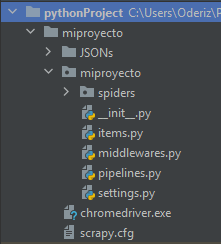
\includegraphics[width=0.4\textwidth]{fig/chromedriver.png}
	\caption[Ruta chromedriver.exe]{Ruta chromedriver.exe}
	\label{fig:ej15}
\end{figure}

En caso de estar en Windows con esto ya es suficiente, aunque al usar Debian son necesarios unos paso más para configurar chromedriver. Los pasos a seguir se muestran en el código \ref{cod:46}.

\begin{lstlisting}[caption={Instrucciones por consola para la configuración de chromedriver en Debian}, label=cod:46]
	#Otorgamos permiso de ejecucion a chromedriver
	sudo chmod +x chromedriver
	
	#Movemos el .exe a directorio /usr/local/share/
	sudo mv chromedriver /usr/local/share/chromedriver
	
	#Creamos la relacion entre el .exe y el directorio
	sudo ln -s /usr/local/share/chromedriver /usr/bin/chromedriver
	
	#Ejecutamos para comprobar si esta bien configurado
	chromedriver --version
	
	#En caso de haber realizado correctamente el proceso deberia aparecer
	una linea parecida a esta
	ChromeDriver 115.0.5790.110
	(5e87dfef0c85687ea835e444d33466745cc0725f-refs/branch-heads/5790_90@{#20})
\end{lstlisting}

\subsubsection{Alternativas probadas}
Antes de saber que es necesario dirigirse a la pagina donde se muestra la gráfica para poder acceder a la página con los datos numéricos, se probo con una Spider que accedía directamente a esta. Visto que el resultado obtenido estaba vacío y, que en apariencia la Spider era correcta, obteniendo teóricamente aquellos datos deseados, se comprobó la web manualmente, resultando en la obtención del error mostrado en la figura \ref{fig:ej5}.\newline
\newline
Es por eso que, partiendo de un uso de Scrapy sin uso de extensiones de terceros, se probó una solución al problema que seguía la metodología de recorrer las webs, de esta manera, se visita inicialmente la web con la gráfica para posteriormente redirigirse a los datos numéricos. Resultando en un nuevo fracaso.\newline
\newline
Esta vez si que se obtenían datos, aunque no de forma correcta, muchas estaciones aparecían repetidas múltiples veces, de tres a siete veces en el peor de los casos visto. Siendo el resultado esperado la aparición de una misma estación un total de dos veces, una con los datos del caudal y otra por los datos del nivel. Tras volver a la comprobación manual, resulto en el mismo comportamiento, por alguna razón, una vez dentro de la web de los datos numéricos, al cambiar el código de la estación y recargar la pagina, lo mismo se actualizaban los datos para mostrar los de la nueva estación como no lo hacían, mostrando los datos de la anterior.\newline
\newline
Esto causó la incertidumbre de si era posible obtener datos la web de forma fiable. Finalmente, tras barajar la posibilidad de pulsar el botón para acceder los datos, se dio con la herramienta usada en la versión final, Selenium y, tiempo después con una alternativa más moderna a esta, Playwright.\newline
\newline
Por suerte, Selenium, al ser usado mediante la extensión scrapy\_selenium, resultó funcionar a la primera, aunque a un costo temporal relativamente alto, en comparación con las demás Spider, con una media de dos minutos y medio de ejecución.\newline
\newline
Al ser código destinado a ejecutarse en intervalos de quince minutos, un tiempo de ejecución así no debería acarrear ningún problema pero, aun y todo, se probó una cuarta alternativa mediante Playwright, al prometer mejoras en los tiempos de ejecución y una mejor optimización.\newline
\newline

\textbf{Playwright}\newline
\newline
Antes que nada, cabe mencionar que Playwright no es compatible con Windows y, tampoco lo es con Debian 11 en su versión actual, resultando ser Debian 11 la versión usada para este proyecto, por lo que no se ha podido llegar a comprobar el funcionamiento del siguiente código, aunque debería ser correcto.

\begin{lstlisting}[caption={Instalación Playwright}, label=cod:47]
	#Instalamos scrapy-playwright
	pip install scrapy-playwright
	
	#Instalamos los navegadores compatibles
	playwright install
\end{lstlisting}

Al ejecutar los comandos del código \ref{cod:47}], se instalaran Playwright junto a sus dependencias necesarias. Si se quiere hacer uso de Playwrith con Scrapy, primero que todo es configurar las dependencias de Playwright, indicándolas mediante \textit{custom\_settings} en una Spider o, si se desea, en settings.py. Como se ve en código \ref{cod:48}.

\begin{lstlisting}[language=Python, caption={Configuración Playwright con Scrapy}, label=cod:48]
	custom_settings = {
		"TWISTED_REACTOR": "twisted.internet.asyncioreactor.AsyncioSelectorReactor",
		"DOWNLOAD_HANDLERS": {
			"https": "scrapy_playwright.handler.ScrapyPlaywrightDownloadHandler",
			"http": "scrapy_playwright.handler.ScrapyPlaywrightDownloadHandler",
		}
	}
\end{lstlisting}

A diferencia de Selenium, Playwright no dispone de un nuevo objeto \textit{Request}, si no que hace uso del \textit{Request} implementado en Scrapy indicándole por argumento que debe usar Playwright. Como se ve en código \ref{cod:49}.

\begin{lstlisting}[language=Python, caption={Playwright basic Request}, label=cod:49]
	yield Request(
		url=url,
		callback=self.parse,
		meta=dict(
			playwright=True,
		),
	)
\end{lstlisting}

\begin{lstlisting}[language=Python, caption={Agua en Navarra Playwright Request}, label=cod:50]
	from scrapy_playwright.page import PageMethod
	
	yield Request(
		url=url,
		callback=self.parse,
		meta=dict(
		playwright=True,
		playwright_page_methods=[
			PageMethod("wait_for_selector", selector="div.botoneraGrafico", state="visible"),
			PageMethod("click", selector="input#btnDatosNumericos"),
			PageMethod("waitForEvent", event="click"),
		],
		),
	)
\end{lstlisting}

Para obtener el comportamiento previsto, la Request configurada se muestra en el código \ref{cod:50}. Los PageMethods indican las acciones a realizar una vez se hace la request, la alternativa optada por Playwright al uso de JavaScript. Primero, espera a que el botón esté cargado dentro de la página, pulsa sobre el y, espera a que la acción de pulsar sea realizada. Según la documentación y los ejemplos estudiados, esta alternativa debería funcionar, pero puesto que no se ha podido ejecutar no es seguro su funcionamiento.

\section{Runners}
Todos los Runners comparten la misma estructura que se explica en código \ref{cod:51}. Posteriormente, se indicará el código de los Runners usados.

\begin{lstlisting}[language=Python, caption={Esctructura básica de un Runner}, label=cod:51]
	from pagina.spiders.pagina_spider import PaginaSpider
	from scrapy.crawler import CrawlerProcess
	from scrapy.utils.project import get_project_settings
	
	
	def main():
		settings = get_project_settings()
		process = CrawlerProcess(settings)
		process.crawl(PaginaSpider)
		process.start()
\end{lstlisting}

El código que compone un Runner se muestra en el código \ref{cod:51}. Primero se incluyen las dependencias, entre ellas la Spider a usar, en caso de querer ejecutar múltiples Spider se deberán importar todas ellas y se ejecutaran en paralelo. En la función \textit{main()}, se toma la configuración del fichero settings.py y en caso de existir de la variable custom\_settings, CrawlerProcess prepara el proceso requerido para ejecutar las Spider, se indica con el método \textit{crawl()} la Spider a usar y, se da comienzo al proceso con \textit{start()}.

\begin{lstlisting}[language=Python, caption={CHCantábrico Data Runner}, label=cod:52]
	from chcantabricoSpider.spiders.chcantabrico_pluvio_spider import ChcantabricoPluvioSpider
	from chcantabricoSpider.spiders.chcantabrico_nivel_spider import ChcantabricoNivelSpider
	from chcantabricoSpider.spiders.chcantabrico_coord_spider import ChcantabricoCoordSpider

	process.crawl(ChcantabricoPluvioSpider)
	process.crawl(ChcantabricoNivelSpider)
	process.crawl(ChcantabricoCoordSpider)
\end{lstlisting}

El código mostrado en \ref{cod:52}, ejecuta ChcantabricoPluvioSpider, ChcantabricoNivelSpider y ChcantabricoCoordSpider.

\begin{lstlisting}[language=Python, caption={CHCantábrico Code Runner}, label=cod:53]
	from chcantabricoSpider.spiders.chcantabrico_code_spider import ChcantabricoCodeSpider

	process.crawl(ChcantabricoCodeSpider)
\end{lstlisting}

El Code Runner de código \ref{cod:53} ejecuta ChcantabricoCodeSpider.

\begin{lstlisting}[language=Python, caption={Aemet Data Runner}, label=cod:54]
	from aemetSpider.spiders.aemet_spider import AemetDataSpider

	process.crawl(AemetDataSpider)
\end{lstlisting}

AemetDataSpider es ejecutada en el código \ref{cod:54}.

\begin{lstlisting}[language=Python, caption={Aemet Code Runner}, label=cod:55]
	from aemetSpider.spiders.aemet_code_spider import AemetCodeSpider
	
	process.crawl(AemetCodeSpider)
\end{lstlisting}

En el código \ref{cod:55} se ejecuta AemetCodeSpider.

\begin{lstlisting}[language=Python, caption={MeteoNavarra Data Runner}, label=cod:56]
	from meteoNavarraSpider.spiders.meteoNavarra_coord_spider import MeteoNavarraCoordSpider
	from meteoNavarraSpider.spiders.meteoNavarra_spider import MeteoNavarraDataSpider

	process.crawl(MeteonavarraDataSpider)
	process.crawl(MeteonavarraCoordSpider)	
\end{lstlisting}

En código \ref{cod:56} se muestra lo necesario para ejecutar MeteoNavarraDataSpider y MeteoNavarraCoordSpider.

\begin{lstlisting}[language=Python, caption={MeteoNavarra Code Runner}, label=cod:57]
	from meteoNavarraSpider.spiders.meteoNavarra_code_spider import MeteoNavarraCodeSpider

	process.crawl(MeteoNavarraCodeSpider)
\end{lstlisting}

MeteoNavarraCodeSpider es ejecutada en el código \ref{cod:57}.

\begin{lstlisting}[language=Python, caption={Agua en Navarra Data Runner}, label=cod:58]
	from aguaEnNavarraSpider.spiders.aguaEnNavarra_data_spider import AguaEnNavarraDataSpider
	
	process.crawl(AguaEnNavarraDataSpider)
\end{lstlisting}

El Code Runner de código \ref{cod:58} ejecuta AguaEnNavarraDataSpider.

\begin{lstlisting}[language=Python, caption={Agua en Navarra Code Runner}, label=cod:59]
	from aguaEnNavarraSpider.spiders.aguaEnNavarra_code_spider import AguaEnNavarraCodeSpider

	process.crawl(AguaEnNavarraCodeSpider)
\end{lstlisting}

El código mostrado en \ref{cod:59}, ejecuta AguaEnNavarraCodeSpider.\newline
\newline
El hecho de que las Spider de obtención de coordenadas se ejecuten junto a las de datos tiene dos motivos, el primero, que son dependientes de los códigos de las estaciones, y como se ejecutan en paralelo sin el JSON con los códigos no funcionan, el segundo, que algunas Spider obtengan los datos a la par que los datos.

\section{Executers}
Los Executers son ficheros bash, estos se reparten en dos secciones, obtención de datos data\_spider\_executer.sh y code\_spider\_executer.sh y, tratamiento de datos data\_work\_executer.sh y code\_work\_executer.sh.

\begin{lstlisting}[caption={Ejecucion de entorno virtual y selección de proyecto Scrapy}, label=cod:60]
	#!/bin/bash
	
	for ((i = 1; i <= $#; i++ )); do
		# Activate the virtual environment
		source Scrapy/${!i}/bin/activate
		
		# Change to the directory containing the Python script
		cd Scrapy/${!i}Spider
		
		# Run the Python script
		
		cd ../..
	done
\end{lstlisting}

Mediante el uso de un bucle se van recorriendo los argumentos pasados en el momento de ejecución. Primero ejecutan el comando para activar el entorno virtual indicada por argumento y se desplazan al directorio del proyecto Scrapy requerido. Para permitir iterar entre los argumentos, una vez ejecutado el script indicado, vuelve al directorio de origen. Se puede ver en código \ref{cod:60}.

\begin{lstlisting}[caption={Ejecución de data\_spider\_runner.py}, label=cod:61]
	# Run the Python script
	python3 data_spider_runner.py
\end{lstlisting}

\begin{lstlisting}[caption={Ejecución de data\_work\_runner.py}, label=cod:62]
	# Run the Python script
	python3 TrabajarJSONs/formatear_data_JSONs.py
	python3 TrabajarJSONs/filtrar_data_JSONs.py
\end{lstlisting}

En caso de data\_spider\_executer.sh, ejecuta el Runner encargado de obtener los datos. Como se ve en el código \ref{cod:61}. code\_spider\_executer.sh, de la misma manera ejecuta el Runner encargado de obtener los códigos. El fichero data\_work\_runner.py, presente en código \ref{cod:62}, ejecuta los script encargados del formateo y filtrado de los datos. Nuevamente, para el caso de code\_work\_runner.py, se realizaría lo mismo, indicando los ficheros para trabajar con los códigos. 

\section{Formateo de datos}
Cada proyecto individual dispone de dos Scripts encargados de formatear los datos, uno para los códigos y otro para los datos per se. El código compartido entre los Script es el primero en ser explicado. Aunque en la explicación se ha usado código de formatear\_data\_JSONs.py, las diferencias respecto a formatear\_code\_JSONs.py se traducen a cambiar nombres de variables y los directorios, la única diferencia radica en la función principal donde se realiza el formateo.

\begin{lstlisting}[language=Python, caption={Declaración variable del JSON que se desea usar}, label=cod:63]
	DataJSON = "datos_pagina.json"
\end{lstlisting}

\begin{lstlisting}[language=Python, caption={Declaración función \textit{openFile()}}, label=cod:64]
	def openFile(filename):
		with open(f'JSONs/RawData/{filename}', "r", encoding="utf-8") as f:
			file = json.loads(f.read())
		return file
\end{lstlisting}

\begin{lstlisting}[language=Python, caption={Declaración función \textit{saveFile()}}, label=cod:65]
	def saveFile(filename, data):
		Path("JSONs/ParsedData").mkdir(parents=True, exist_ok=True)
		with open(f'JSONs/ParsedData/{filename}', 'w', encoding='utf-8') as outfile:
			json.dump(data, outfile)
\end{lstlisting}

\begin{lstlisting}[language=Python, caption={Declaración función \textit{main()}}, label=cod:66]
	def main():
		file = openFile(DataJSON)
		formatData(file)
\end{lstlisting}

Una variable que indica el nombre o la ruta del fichero a leer, siguiendo el ejemplo de código \ref{cod:63}; una función para abrir los ficheros, como en código \ref{cod:64}; otra función para crear el directorio de guardado en caso de no existir y guardar los ficheros, mostrada en código \ref{cod:65} y una función \textit{main()} para iniciar el proceso, visible en código \ref{cod:66}. Con el fin de aligerar la explicación de la función principal, \textit{formatData()}, se va a explicar inicialmente el funcionamiento base de esta, código \ref{cod:67}.

\begin{lstlisting}[language=Python, caption={Declaración función base \textit{formatData()}, concretamente esta versión es usada para formatear los datos de Aemet}, label=cod:67]
	def formatData(file):
		formattedJSON = []
		for line in file:
			datos = []
			for data in line['datos']:
				dato = {
					'fecha y hora': datetime.strptime(data['fecha y hora'], "%d/%m/%Y %H:%M:%S").strftime("%Y-%m-%d %H:%M"),
					'temperatura (C)': data['temperatura (C)'],
					'humedad (%)': data['humedad (%)'],
					'precipitacion (mm)': data['precipitacion (mm)'],
					'nivel (m)': None,
					'caudal (m^3/s)': None,
					'radiacion (W/m^2)': None,
				}
				datos.append(dato)
			header = {
				'estacion': line['estacion'],
				'datos': datos
			}
			formattedJSON.append(header)
		saveFile(DataJSON, formattedJSON)
\end{lstlisting}

La función del código \ref{cod:67}, recibe como argumento el archivo de datos con el que trabajar, file; crea una lista vacía para almacenar el JSON formateado, formattedJSON; itera por cada estación en el fichero; itera por los datos de las estaciones, creando con ellos objetos JSON, dato, con el formato deseado, la temperatura antes de almacenarse se convierte de String a DateTime con el uso de \textit{strptime()} y posteriormente se cambia al formato usado por PosrGreSQL con \textit{strftime()}, los datos que no se dispongan se ponen a None; almacena cada objeto en la lista datos; cuando terminan los datos de una estación, crea un segundo objeto JSON, header, en el que se almacena el código y los datos de esta. Finalmente se incluyen en formattedJSON hasta terminar con todas las estaciones y se guarda el fichero.\newline
\newline
MeteoNavarra, dispone de un formateo de datos en bruto peculiar, pudiendo aparecer la misma estación múltiples veces, es por eso, que se ha definido la función del código \ref{cod:68}.

\begin{lstlisting}[language=Python, caption={Declaración función \textit{unifyData()} para el correcto funcionamiento del formateo de MeteoNavarra}, label=cod:68]
	def unifyData(dataFile, cod):
		datos = []
		for line in dataFile:
			if line['estacion'] == cod:
				for dato in line['datos']:
					datos.append(dato)
		
		unifiedData = {
			'estacion': cod,
			'datos': datos
		}
		return unifiedData
\end{lstlisting}

Lo que hace el código \ref{cod:68} es, recorrer las estaciones en busca de aquella que comparta el mismo código y crea un nuevo diccionario con los datos de esta estación, posteriormente devuelve el diccionario.

\begin{lstlisting}[language=Python, caption={Paso inicial en la función \textit{formatData()} de MeteoNavarra}, label=cod:69]
	codes = [x["estacion"] for x in file]
	uniqueCodes = pd.Series(codes).drop_duplicates().tolist()
	unifiedJSON = []
	for code in uniqueCodes:
		data = unifyData(file, code)
		unifiedJSON.append(data)
\end{lstlisting}

Antes de realizar el procedimiento del código \ref{cod:67}, se incluye el código \ref{cod:69}, se obtiene una lista de todos los códigos de estación; con el uso del objeto \textit{Series} de pandas, elimina la duplicidad con \textit{drop\_duplicates()} y lo vuelve a convertir en una lista, \textit{tolist()}. Luego itera por los códigos mientras llama a la función \textit{unifyData()} y almacena el resultado en unifiedJSON.\newline
\newline
CHCantábrico y Agua en Navarra comparten la misma estructuración de Script. CHCantábrico por tener los datos en dos ficheros y Agua en Navarra por el formato de los datos recibido de la web, apareciendo dos veces cada estación dentro del JSON, pero a diferencia de MeteoNavarra, una con los datos del caudal y otra con los de nivel.

\begin{lstlisting}[language=Python, caption={Declaración función \textit{searchEstacionData()}, especifica en el formateo de datos de CHCantábrico y Agua en Navarra}, label=cod:70]
	def searchEstacionData(code, dataFile1=[], dataFile2=[]):
		datos = []
		for data in dataFile1:
			if data['estacion'] == code:
				datos.append(data)
		for data in dataFile2:
			if data['estacion'] == code:
				datos.append(data)
		return datos
\end{lstlisting}

\textit{searchEstacionData()}, en código \ref{cod:70}, se encarga de recibir de uno a dos ficheros y generar un diccionario JSON con todos los datos encontrados de una misma estación, para ello recorre los ficheros estación por estación comparando los códigos y en caso de coincidir se guardan en la variable datos, la cual se devolverá al final.

\begin{lstlisting}[language=Python, caption={Declaración función \textit{searchDateData()}}, label=cod:71]
	def searchDateData(dataFile, date):
		for data in dataFile:
			if data['fecha y hora'] == date:
				return data
\end{lstlisting}

La función en código \ref{cod:71}, asegura que la fecha de los datos obtenidos de los JSON coincidan, iterando por los datos en busca de la fecha que coincida y devolver el dato correspondiente. \newline
\newline
Como el código en la función \textit{formatData()} es virtualmente el mismo, se explicará el caso de CHCantábrico.

\begin{lstlisting}[language=Python, caption={Lectura de los ficheros de datos de CHCantábrico}, label=cod:72]
	levelDataFile = openFile('datos_nivel_chcantabrico.json')
	pluvioDataFile = openFile('datos_pluvio_chcantabrico.json')
\end{lstlisting}

En este caso, el fichero que recibe la función \textit{formatData()} es el de los códigos de estación, es por eso que lo primero a hacer en la función es abrir los ficheros con los datos. Como se ve en \ref{cod:72}.

\begin{lstlisting}[language=Python, caption={Dentro del bucle que itera por estaciones, obtención de los datos de la estacion y declaración de indices}, label=cod:73]
	lineData = searchEstacionData(line['codigo'], levelDataFile, pluvioDataFile)
	index = 0
	indexSecundario = 1
	if len(lineData) == 2:
		if len(lineData[0]) < len(lineData[1]):
			index = 1
			indexSecundario = 0
\end{lstlisting}

Dentro del bucle principal, se llama a \textit{searchEstacionData()} para obtener los datos de ambos ficheros en una única lista \ref{cod:74}, lineData; index e indexSecundario representan los elementos presentes en esta, que, en caso de tener dos instancias de una misma estación, se comprueba cual es más extensa para indicar la instancia principal. Se hace así ya que no siempre aparecen la misma cantidad de datos, de esta forma, trabajar aquel con más datos hace que sea menos probable dejar datos sin tratar. Se puede ver en código \ref{cod:73}.

\begin{lstlisting}[language=Python, caption={Formato del diccionario lineData en caso de disponer de dos instancias de una misma estación}, label=cod:74]
	[
		[
			estacion: ...
			datos: [...]
		],
		[
			estacion: ...
			datos: [...]
		],
	]
\end{lstlisting}

\begin{lstlisting}[language=Python, caption={Modificación del bucle interno de \textit{formatData()}}, label=cod:75]
	for data in lineData[index]['datos']:
		dato = {
			'fecha y hora': datetime.strptime(data['fecha y hora'], "%d/%m/%Y %H:%M:%S").strftime("%Y-%m-%d %H:%M"),
			'temperatura (C)': None,
			'humedad (%)': None,
			'precipitacion (mm)': None,
			'nivel (m)': None,
			'caudal (m^3/s)': None,
			'radiacion (W/m^2)': None,
		}
\end{lstlisting}

Trabajar con lineData supone tener que cambiar el bucle interno de \textit{formatData()}, mostrado en el código \ref{cod:75}. El bucle se realiza indicando el indice de la instancia principal y, excepto la hora, todos los datos son indicados como None. Posteriormente, aun dentro del bucle, se incluyen los datos con el código \ref{cod:76}.

\begin{lstlisting}[language=Python, caption={Inclusion de los datos en el objeto JSON dato}, label=cod:76]
		if 'nivel (m)' in data:
			dato['nivel (m)'] = data['nivel (m)']
		elif 'precipitacion (mm)' in data:
			dato['precipitacion (mm)'] = data['precipitacion (mm)']
		
		if len(lineData) == 2:
			dateData = searchDateData(lineData[indexSecundario]['datos'], data['fecha y hora'])
			try:
				if 'nivel (m)' in dateData:
					dato['nivel (m)'] = dateData['nivel (m)']
				if 'precipitacion (mm)' in dateData:
					dato['precipitacion (mm)'] = dateData['precipitacion (mm)']
			except TypeError:
				pass
\end{lstlisting}

Primero comprueba que tipo de dato esta presente en los datos de instancia principal y, guarda el dato presente; luego, en caso de existir una segunda instancia, llama a \textit{searchDateData()} para buscar el dato correspondiente a la fecha en la instancia secundaria; si no se recibe el error \textit{TypeError}, pues indicaría que no existe registro para esa fecha sobre la instancia secundaria, realiza nuevamente la comprobación de tipo y lo guarda. El código \ref{cod:76} corresponde a la explicación.\newline
\newline
El código \ref{cod:78} de formateo de códigos de estación es el mismo para todas las webs, con la excepción de CHCantábrico y MeteoNavarra, que obtiene las coordenadas abriendo el fichero correspondiente con \textit{openFile()} y las buscan con \textit{searchEstacionCoords()}.

\begin{lstlisting}[language=Python, caption={Declaración función \textit{searchEstacionCoords()}} usada para formatear los JSON de códigos en CHCantábrico y MeteoNavarra, label=cod:77]
	def searchEstacionCoords(code, coordFile):
		for data in coordFile:
			if data['estacion'] == code:
				return data['coordenadas']
\end{lstlisting}

En ella se recibe el código de la estación a buscar y el fichero con las coordenadas, se itera sobre el y en caso de encontrar una estación con el mismo código enviado, re devuelven las coordenada. En caso de no encontrar la estación, al no especificar un \textit{return}, la variable se quedara como None. Visible en código \ref{cod:77}.

\begin{lstlisting}[language=Python, caption={Declaración función \textit{formatCode()}}, label=cod:78]
	def formatCode(file):
		formattedJSON = []
		for line in file:
			header = {
				'estacion': line['descripcion'],
				'codigo': line['estacion'],
				'coordenadas': line['coordenadas'],
				'seguimiento': None,
				'prealerta': None,
				'alerta': None,	
			}
			formattedJSON.append(header)
		saveFile('codigos_aguaEnNavarra.json', formattedJSON)
\end{lstlisting}

\section{Filtrado de datos}
El siguiente paso a realizar, es el filtrado de los JSON por el script filtras\_data\_JSONs.py y filtras\_code\_JSONs.py

\begin{lstlisting}[language=Python, caption={Declaración rutas JSONs y nombre de fichero}, label=cod:79]
	OldDir = "JSONs/OldData/"
	ParsedDir = "JSONs/ParsedData/"
	RefinedDir = "JSONs/RefinedData/"
	DataJSON = "datos_aemet.json"
\end{lstlisting}

\begin{lstlisting}[language=Python, caption={Declaración función openFile()}, label=cod:80]
	def openFile(fileDir):
		try:
			with open(fileDir + DataJSON, "r", encoding="utf-8") as f:
				file = json.loads(f.read())
		except FileNotFoundError:
			file = None
		return file
\end{lstlisting}

Se declaran las variables representativas de las rutas y el nombre del fichero JSON. Como se muestra en código \ref{cod:79}. La función en código \ref{cod:80}, prueba a abrir el fichero anteriormente declarado (datos\_aemet.json) sobre la ruta indicada (fileDir), en caso de no existir, se marca el fichero como None, finalmente devuelve el fichero. El tratado de la excepción FileNotFoundError se realiza pensada en la primera vez que se haga uso de la plataforma, ya que esta no dispondría de datos posteriores con los que hacer una comparación.

\begin{lstlisting}[language=Python, caption={Declaración función saveFile()}, label=cod:81]
	def saveData(jsonDir, DataFile):
		Path(jsonDir).mkdir(parents=True, exist_ok=True)
		with open(jsonDir + DataJSON, 'w', encoding='utf-8') as outfile:
			json.dump(DataFile, outfile)
\end{lstlisting}

Recibiendo como argumento el directorio sobre el que se desea guardar el fichero (jsonDir) y un diccionario JSON con los datos a guardar (DataFile), esta función, comprueba la existencia del directorio y en caso de no hacerlo lo crea. Tras ello, guarda los datos en el directorio con el uso de \textit{json.dump()}. Función en código \ref{cod:81}.

\begin{lstlisting}[language=Python, caption={Declaración función searchEstacionData()}, label=cod:82]
	def searchEstacionData(code, dataFile):
		for data in dataFile:
			if data['estacion'] == code:
				return data["datos"]
\end{lstlisting}

Como no es seguro que los datos recibidos estén siempre en el mismo orden, se ha definido esta función para asegurarse de trabajar siempre con los datos de la estación correcta. Recorre el fichero viejo y cuando encuentra la estación con el mismo código devuelve los datos de esta. Función mostrada en código \ref{cod:82}.

\begin{lstlisting}[language=Python, caption={Declaración rutas JSONs}, label=cod:84]
	def main():
		newFile = openFile(ParsedDir)
		oldFile = openFile(OldDir)
		
		if oldFile is None:
			saveData(RefinedDir, newFile)
			saveData(OldDir, newFile)
			return
		
		refineData(newFile, oldFile)
		saveData(OldDir, newFile)
\end{lstlisting}

La función \textit{main()}, vista en código \ref{cod:84}, abre los ficheros indicados en las rutas ParsedDir y OldDir, en caso de que oldFile sea None, guarda los datos refinados en el directorio refinedDir, el fichero con los datos nuevos pasa al directorio OldDir y en el programa finaliza. Si se dispone de datos en oldFile, llama a \textit{refineData()} y posteriormente se marca newFile como viejo al guardarlo en OldDir.

\begin{lstlisting}[language=Python, caption={Declaración función refinedData()}, label=cod:83]
	def refineData(newFile, oldFile):
		refinedFile = []
		
		for i, item in enumerate(newFile):
			newData = []
			oldData = searchEstacionData(item['estacion'], oldFile)
			for data in item["datos"]:
				if data["fecha y hora"] not in [x["fecha y hora"] for x in oldData]:
					newData.append(data)
		if newData:
			refinedFile.append(
				{
					"coordenadas": item["coordenadas"],
					"estacion": item["estacion"],
					"datos": newData
				}
			)
		
		saveData(RefinedDir, refinedFile)
\end{lstlisting}

La función \textit{refinedData()} en código \ref{cod:83}, se encarga de la comparación de los ficheros, recibidos en los argumentos newFile y oldFile. Empezando con la explicación, se define la lista vacía refinedFile, encargada de almacenar los datos nuevos de todas las estaciones; se itera por cada estación en newFile; se define una segunda lista newData para almacenar los nuevos datos por estación; se llama a \textit{searchEstacionData()} para buscar los datos viejos de la estación; se itera por todos los datos de los presentes en la estación; se comprueba que no exista previamente en los datos de esa misma estación en oldData; en caso de que el dato no este presente, se almacena en newData; si existe algún dato nuevo (newData no esta vacía), se crea un objeto JSON que sigue la estructuración definida para los ficheros de datos y, se almacena en refinedData; finalmente los datos se guardan en un fichero en la ruta especificada RefinedDir.

\begin{lstlisting}[language=Python, caption={Declaración función refinedCode()}, label=cod:114]
	def refineCode(newFile, oldFile):
		refinedFile = []
		
		for item in newFile:
			newCode = []
			if item["codigo"] not in [x["codigo"] for x in oldFile]:
				newCode.append(item)
		
		saveCode(RefinedDir, refinedFile)
\end{lstlisting}

En el código \ref{cod:114}, se puede ver la implementación de la función \textit{refineCode()}, la cual recorre el fichero de códigos buscando si existe alguna nueva estación. El resto de funciones usadas tienen la misma implementación que para filtras\_datos\_JSONs.py.

\section{Posts}
Como Posts, se hace referencia a los Scripts code\_post.py y data\_post.py. Como ambos comparten la misma codificación se explicaran de forma general y, se mostraran las diferencias.

\begin{lstlisting}[language=Python, caption={Declaración variables code\_post.py}, label=cod:85]
	url = "http://localhost:8000/appAPI/storeCode"
	
	with open(f"JSONs/ParsedCode/codigos_{sys.argv[1]}.json", encoding="utf-8") as f:
		data = json.load(f)
\end{lstlisting}

\begin{lstlisting}[language=Python, caption={Declaración variables data\_post.py}, label=cod:86]
	url = "http://localhost:8000/appAPI/storeData"
	
	with open(f"JSONs/ParsedData/datos_{sys.argv[1]}.json", encoding="utf-8") as f:
		data = json.load(f)
\end{lstlisting}

\begin{lstlisting}[language=Python, caption={Llamada POST}, label=cod:87]
	headers = {'content-type': 'application/json'}
	r = requests.post(url, json=data, headers=headers)
\end{lstlisting}

Se declara la URL a la que se desea hacer la llamada y, se lee el fichero que se ha indicado al pararlo por argumento a la hora de ejecutar el Script. como se muestra en los códigos \ref{cod:85} y \ref{cod:86}. Finalmente, se indica en headers el tipo de contenido que dispone la llamada, en este caso JSON y, se realiza la llamada con el método \textit{post()} proporcionado por la librería requests, como en código \ref{cod:87}.

\section{Cron}
Dentro del archivo crontab se han definido los comandos presentes en código \ref{cod:103}. Estos representan las rutinas de ejecución, ejecutando cada quince minutos el código relacionado con los datos de las estaciones de Agua En Navarra y CHCantábrico; cada treinta minutos el de MeteoNavarra; cada hora el de Aemet y cada primeros de mes se ejecutará el código para la obtención de códigos de estación para comprobar si ha habido algún cambio en estas.

\begin{lstlisting}[caption={Trabajos configurados para ser ejecutados por Cron}, label=cod:103]
	#Cada 15 minutos
	*/15 * * * * data_spider_executer.sh aguaEnNavarra chcantabrico
	*/15 * * * * data_work_executer.sh aguaEnNavarra chcantabrico
	*/15 * * * * data_post.py aguaEnNavarra chcantabrico
	
	#Cada 30 minutos
	*/30 * * * * data_spider_executer.sh meteoNavarra
	*/30 * * * * data_work_executer.sh meteoNavarra
	*/30 * * * * data_post.py meteoNavarra
	
	#Cada hora
	0 * * * * data_spider_executer.sh aemet
	0 * * * * data_work_executer.sh aemet
	0 * * * * data_post.py aemet

	#Cada primeros del mes a las 03:00
	0 3 1 * * code_spider_executer.sh aguaEnNavarra chcantabrico aemet meteoNavarra
	0 3 1 * * code_work_executer.sh aguaEnNavarra chcantabrico aemet meteoNavarra
	0 3 1 * * code_post.py aguaEnNavarra chcantabrico aemet meteoNavarra
\end{lstlisting}

Todo el código realizado esta disponible en \url{https://github.com/ArkaitzOderiz/ScrapyScraping}.